\documentclass[conference]{IEEEtran}
\IEEEoverridecommandlockouts
% The preceding line is only needed to identify funding in the first footnote. If that is unneeded, please comment it out.
\usepackage[square]{natbib}
\setcitestyle{numbers}
\usepackage{amsmath,amssymb,amsfonts}
\usepackage{algorithmic}
\usepackage{graphicx}
\usepackage{textcomp}
\usepackage{cleveref}
\usepackage{xcolor}
\def\BibTeX{{\rm B\kern-.05em{\sc i\kern-.025em b}\kern-.08em
    T\kern-.1667em\lower.7ex\hbox{E}\kern-.125emX}}
\begin{document}
  
  \title{Reinforcement learning for self driving taxis}
  
  \author{\IEEEauthorblockN{Daniel Aaron Salwerowicz}
    \IEEEauthorblockA{\textit{Institutt for datateknologi og beregningsorienterte ingeniørfag} \\
      \textit{Arctic University of Norway, Narvik}\\
      Narvik, Norway \\
      dsa014@post.uit.no}
  }

\maketitle

\begin{abstract}
  In this report I describe my research related to developing a system with self driving taxis that operate in an imaginary city picking up passengers after cinema, opera, and restaurant close.
\end{abstract}

\begin{IEEEkeywords}
  Reinforcement learning, Roth Erev, Q-learning, Multi Agent Systems
\end{IEEEkeywords}

\section{Introduction}


\section{Problem specification}


\section{Methods applied}


\section{Results}

%\begin{table}[htbp]
%  \centerline{
%    \begin{tabular}{l l}
%      Parameter    & Value \\
%      Conv. kernel & 3x3   \\
%      Conv. stride & 1x1   \\
%      Pool. size   & 2x2   \\
%      1st dropout  & 0.5   \\
%      2nd dropout  & 0.3   \\
%      3rd dropout  & 0.5   \\
%      4th dropout  & 0.3   \\
%      Epochs       & 200   \\\\
%  \end{tabular}}
%  \caption{Parameter values for categorizing pictures in CIFAR-10 dataset.}
%  \label{tab:parametersCIFAR}
%\end{table}


%\begin{figure}[htbp]
%  \centerline{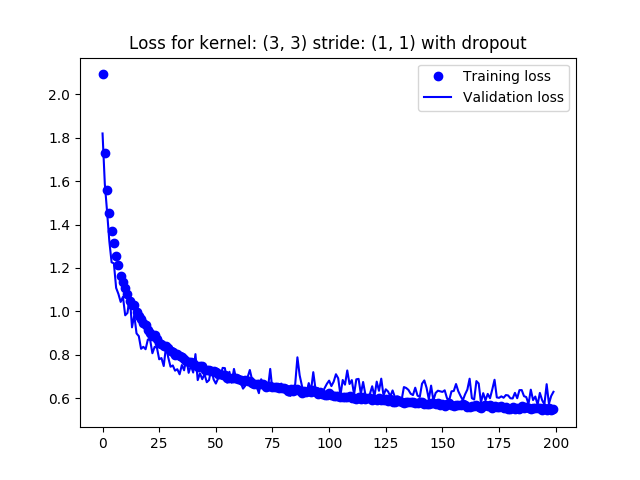
\includegraphics[width=.4\textwidth]{Best_Loss}}
%  \centerline{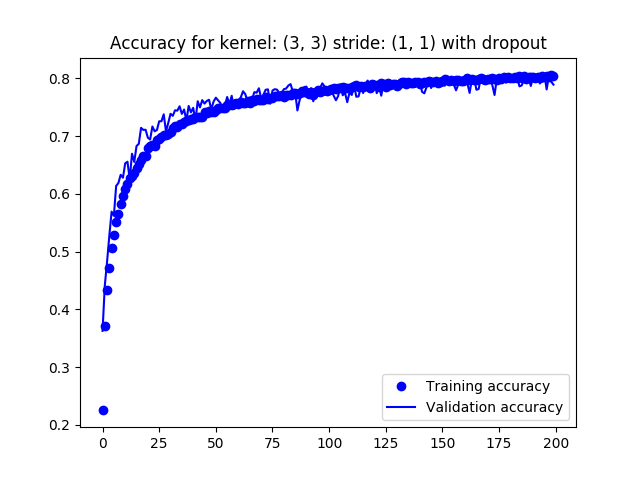
\includegraphics[width=.4\textwidth]{Best_Accuracy}}
%  \caption{Loss and Accuracy graphs (respectively) for the training and validation data reached by my CNN on CIFAR-10 dataset.}
%  \label{fig:LossAccCIFAR}
%\end{figure}
\section{Discussion}



\section*{Acknowledgments}
I would like to thank Christopher Kragebøl Hagerup, Kent Arne Larsen, Hans Victor Andersson Lindbäck, and Olav Kjartan Larseng for helping me underway. We brainstormed a lot of ideas on how to solve this problem, and I got a lot of help with task 1.3 from Victor.

\bibliographystyle{apalike}
\bibliography{Bibliography}

\end{document}

